\section{Simulation Results} \label{sec:res}
The proposed HRDNUT latch has been implement using the 1.05V 32nm PTM library \cite{PTM} and simulated in HSPICE. All transistors were set to the minimum size with the PMOS widths set to W=80nm and the NMOS widths set to W=40nm. To evaluate the DNU reliability of the design, current pulses were injected for every possible error combination. The injection current was calculated using the equation found in \cite{injeq}. The equation is given below with $\tau$ as the technology dependent constant, $Q_o$ as the injection current value and $t$ as the variable for time. 

\begin{equation}\label{qeq}
I(t)=\frac{2Q_o}{\tau\sqrt{\pi}}\sqrt{\frac{t}{\tau}}e^{\frac{-t}{\tau}}
\end{equation}

Using equation (\ref{qeq}) $\tau$ was set to $32\times10^{-12}$ and $Q_o$ was set to $5\text{fC}$. In all simulations, the latch was operated at a frequency of 1Ghz. In Figs. \ref{fig:CLK}-\ref{fig:n5n6}, we present the waveforms for each case discussed in Section \ref{Proposed} and show that the HRDNUT is fully capable of recovering all nodes in the presence of a DNU. 

\begin{figure}[!htbp]
\centering
\parbox{4cm}{
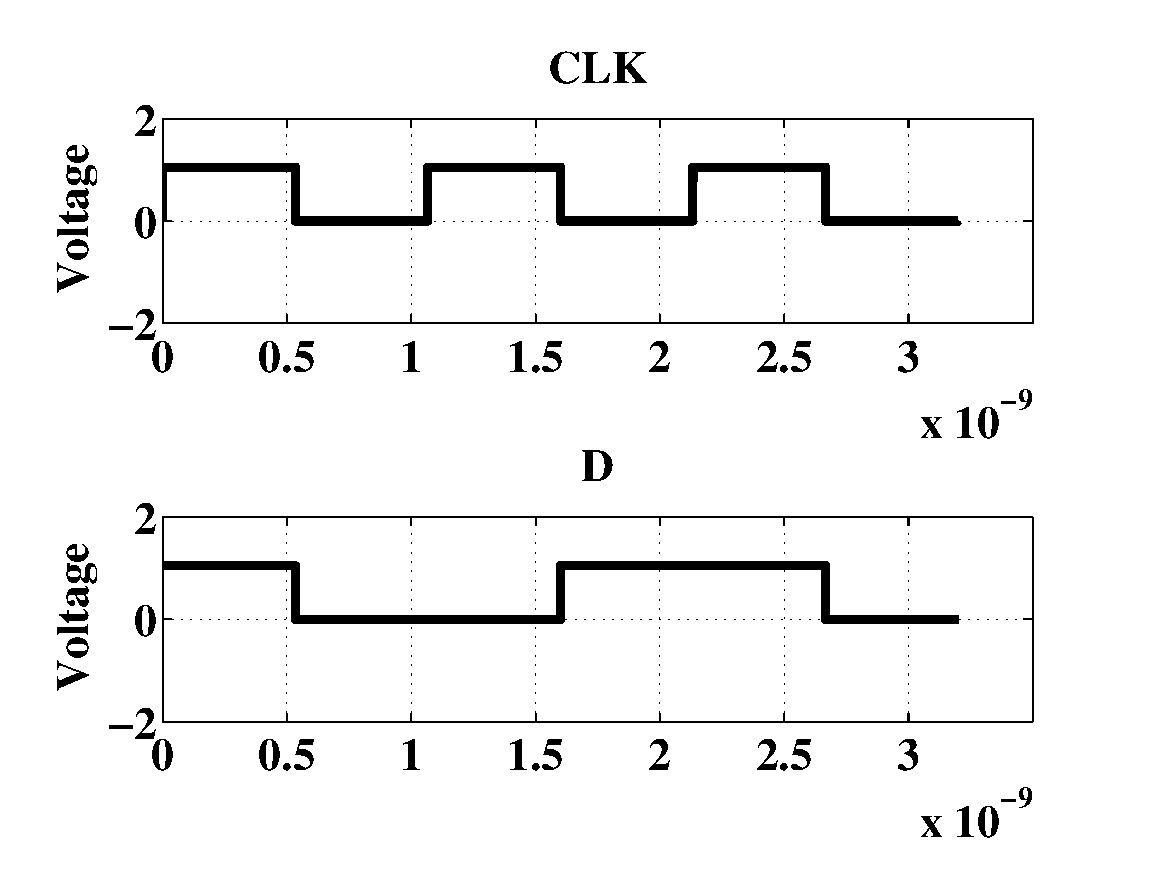
\includegraphics[width=1.15\linewidth]{Figures/WavePlots/CLKD.eps}
\caption{Waveforms for CLK and D.}
\label{fig:CLK}}
\qquad
\begin{minipage}{4cm}
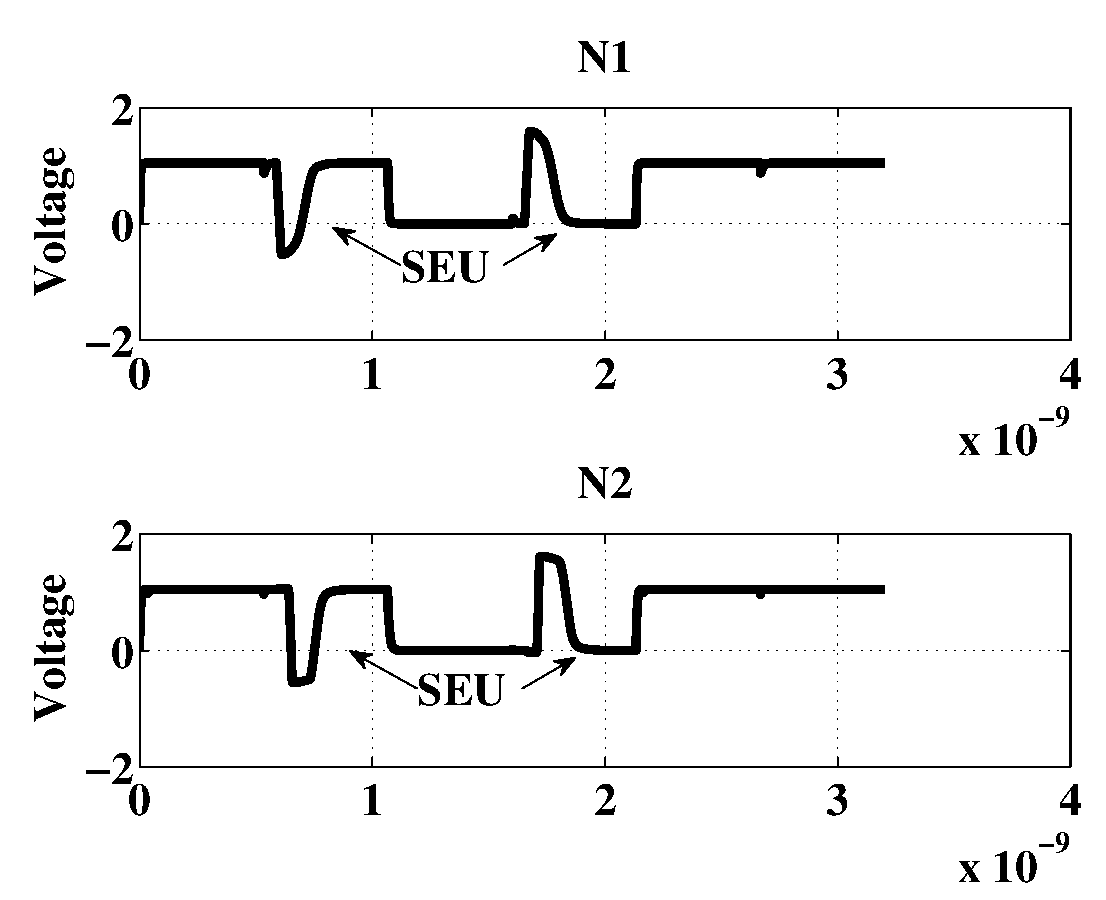
\includegraphics[width=\linewidth]{Figures/WavePlots/n1n2.eps}
\caption{Node pair n1 and n2 upset and recovery.}
\label{fig:n1n2}
\end{minipage}
\end{figure}

\begin{figure}[!htbp]
\centering
\parbox{4cm}{
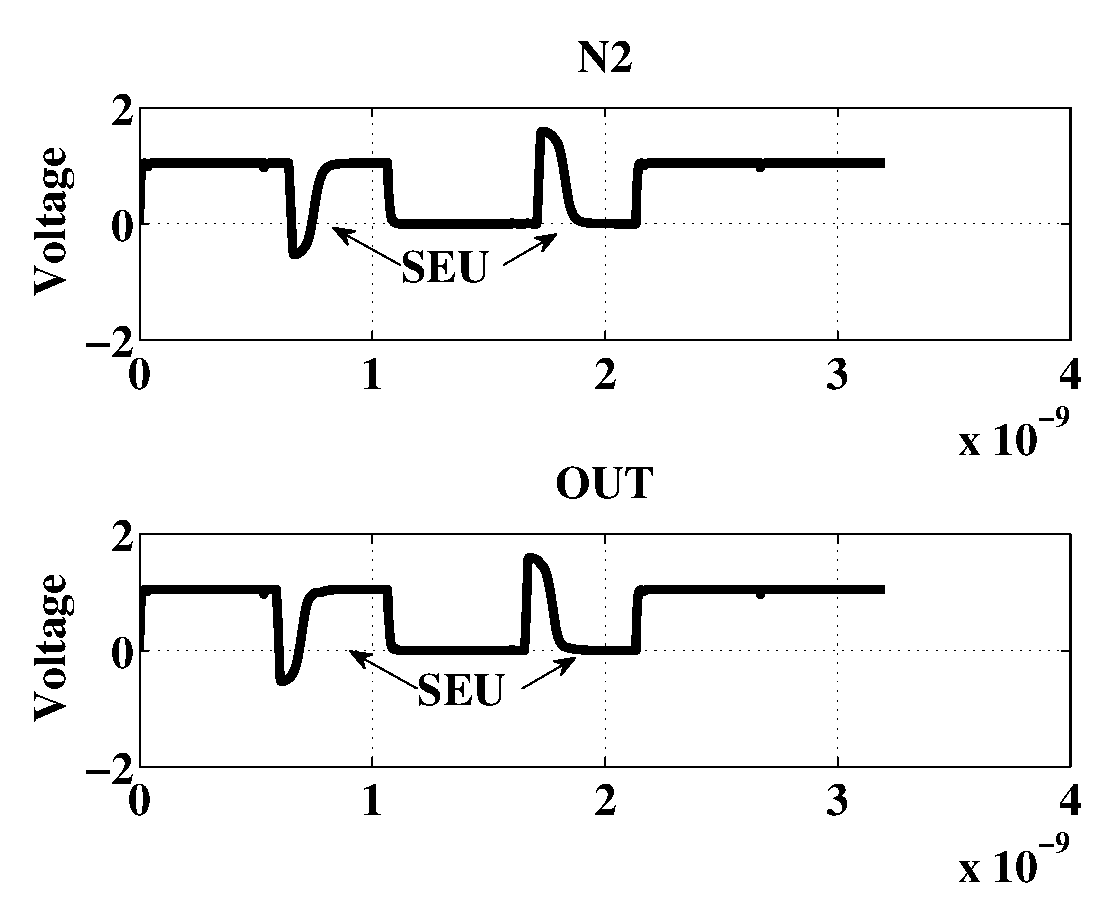
\includegraphics[width=\linewidth]{Figures/WavePlots/n2out.eps}
\caption{Node pair n2 and out upset and recovery.}
\label{fig:n2out}}
\qquad
\begin{minipage}{4cm}
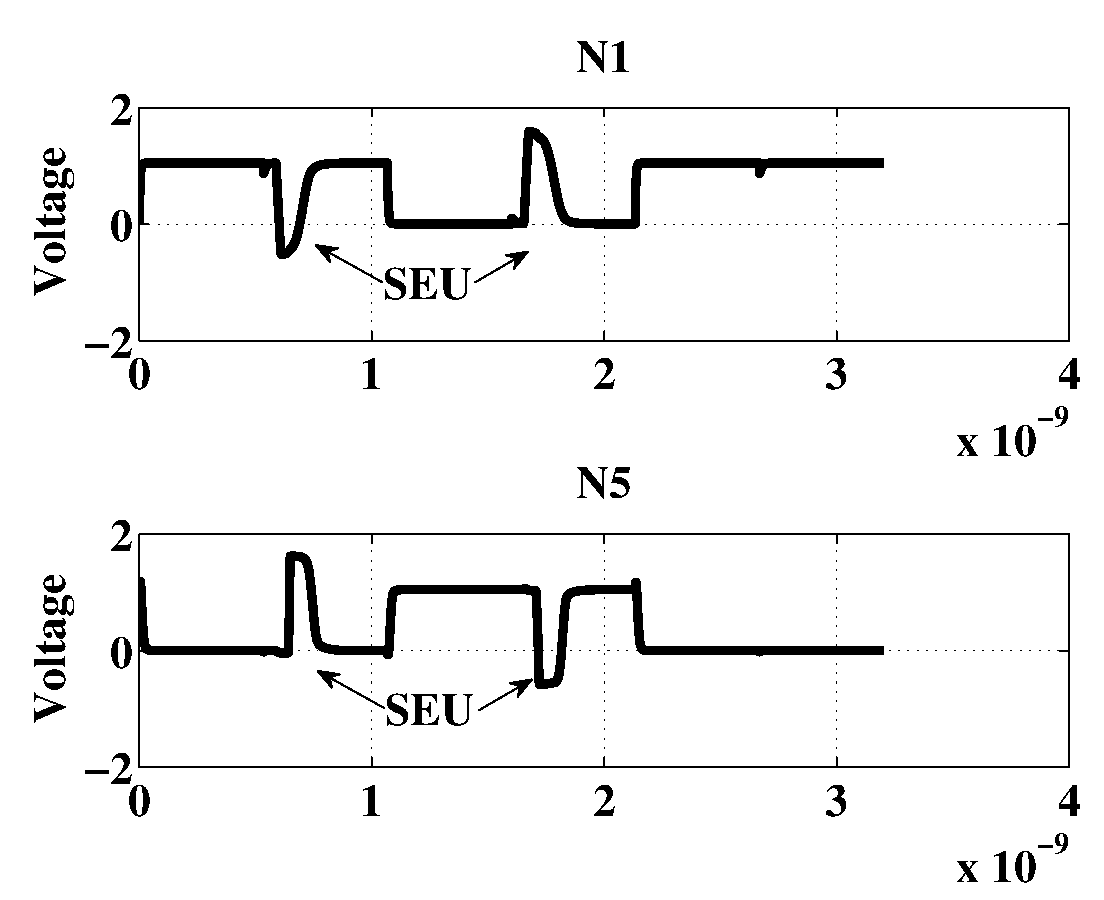
\includegraphics[width=\linewidth]{Figures/WavePlots/n1n5.eps}
\caption{Node pair n1 and n5 upset and recovery.}
\label{fig:n1n5}
\end{minipage}
\end{figure}

\begin{figure}[!htbp]
\centering
\parbox{4cm}{
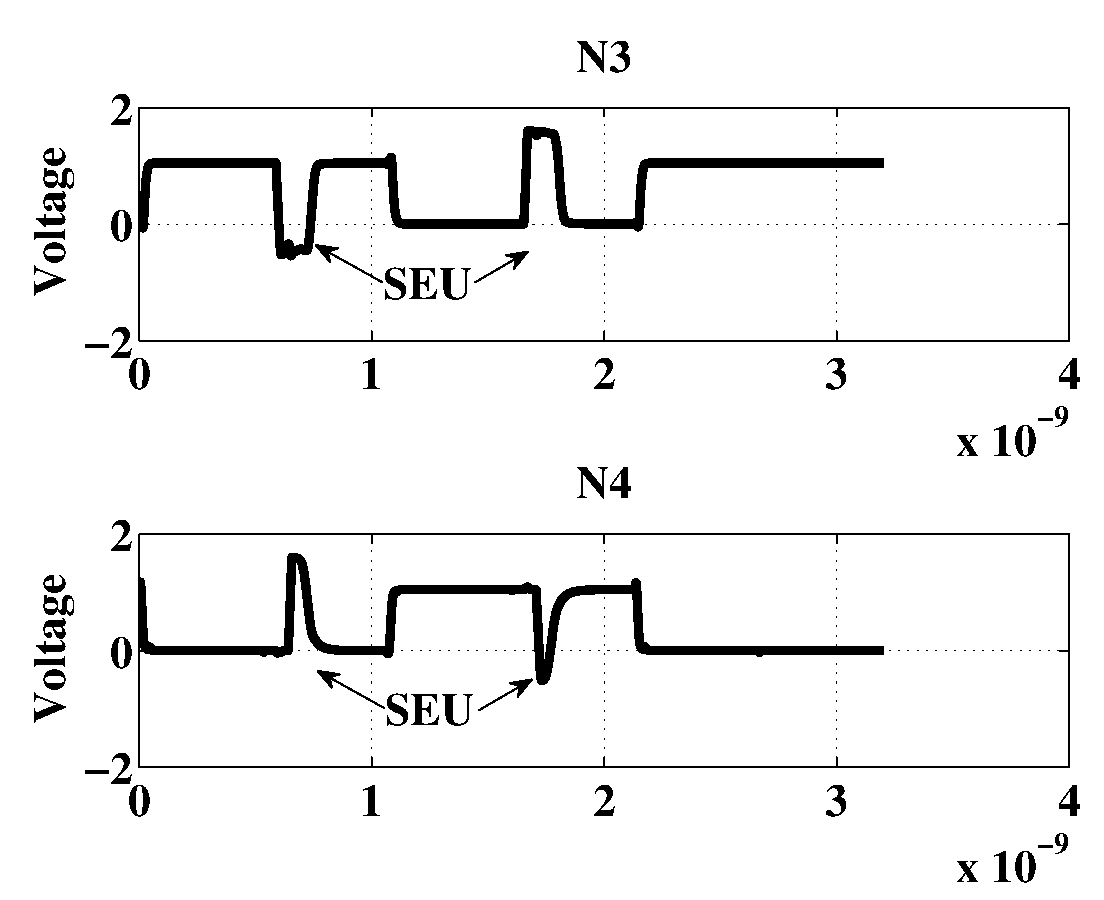
\includegraphics[width=\linewidth]{Figures/WavePlots/n3n4.eps}
\caption{Node pair n3 and n4 upset and recovery.}
\label{fig:n3n4}}
\qquad
\begin{minipage}{4cm}
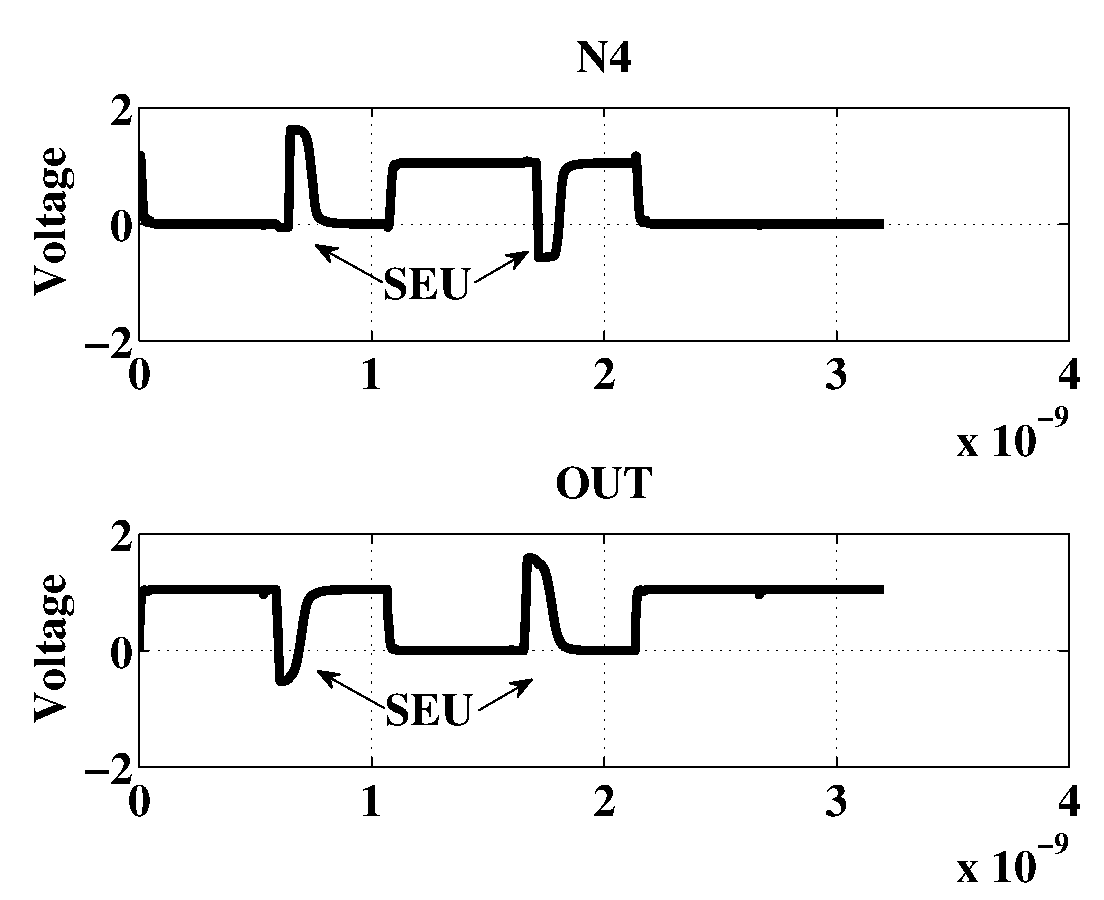
\includegraphics[width=\linewidth]{Figures/WavePlots/n4out.eps}
\caption{Node pair n4 and out upset and recovery.}
\label{fig:n4out}
\end{minipage}
\end{figure}

\begin{figure}[!htbp]
\centering
\parbox{4cm}{
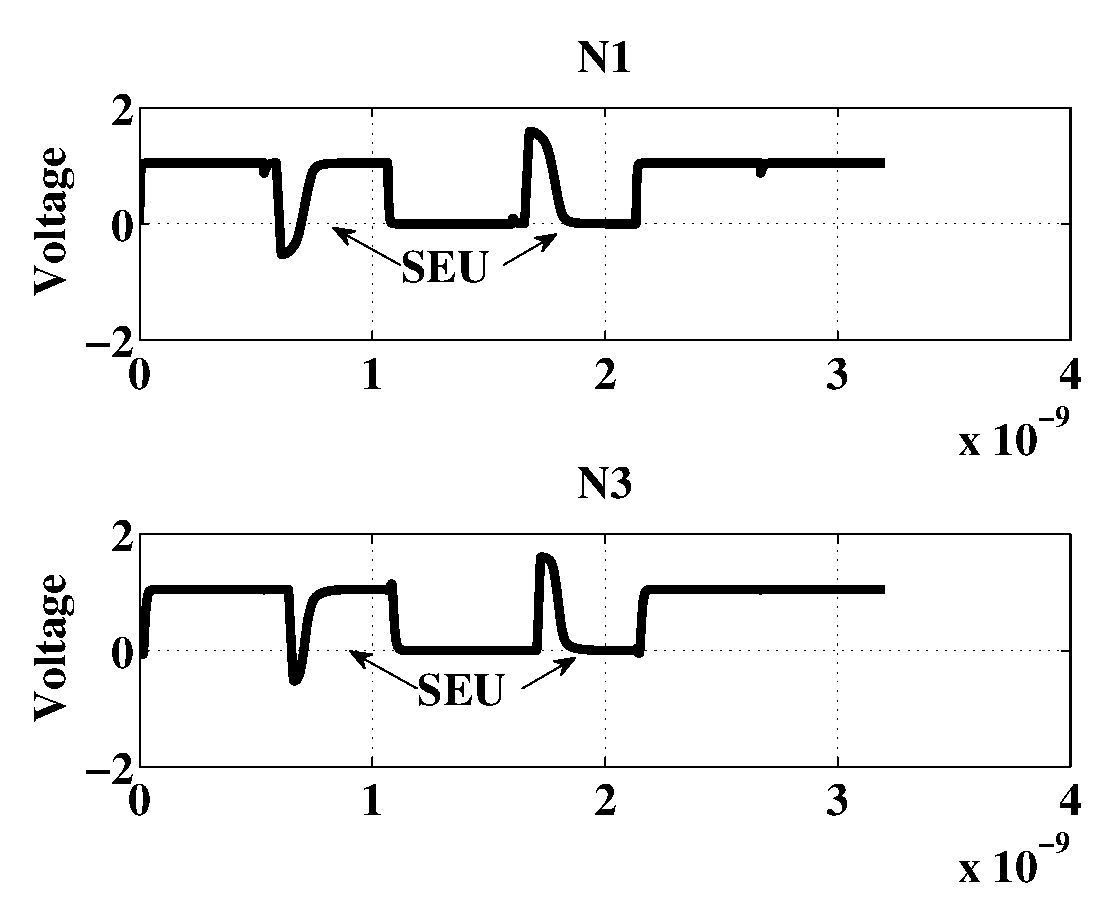
\includegraphics[width=\linewidth]{Figures/WavePlots/n1n3.eps}
\caption{Node pair n1 and n3 upset and recovery.}
\label{fig:n1n3}}
\qquad
\begin{minipage}{4cm}
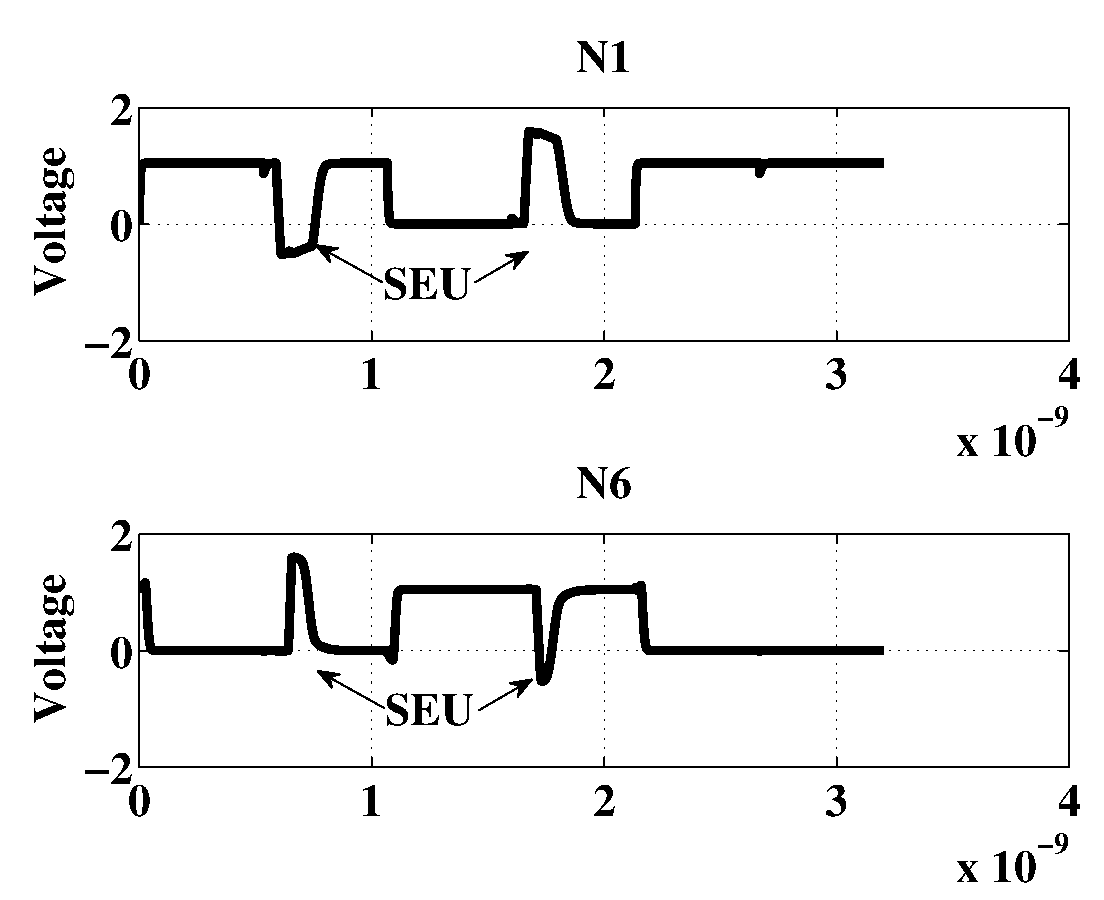
\includegraphics[width=\linewidth]{Figures/WavePlots/n1n6.eps}
\caption{Node pair n1 and n6 upset and recovery.}
\label{fig:n1n6}
\end{minipage}
\end{figure}

\begin{figure}[!htbp]
\centering
\parbox{4cm}{
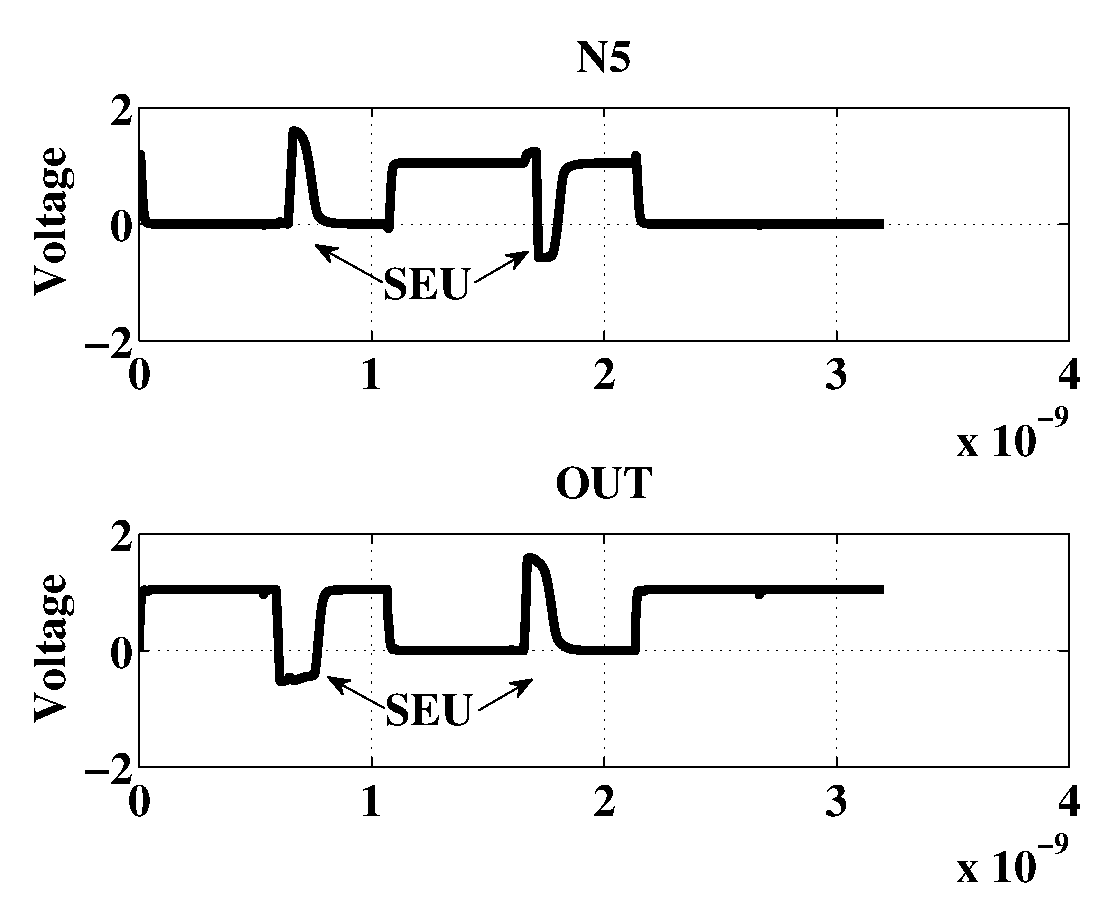
\includegraphics[width=\linewidth]{Figures/WavePlots/n5out.eps}
\caption{Node pair n5 and out upset and recovery.}
\label{fig:n3out}}
\qquad
\begin{minipage}{4cm}
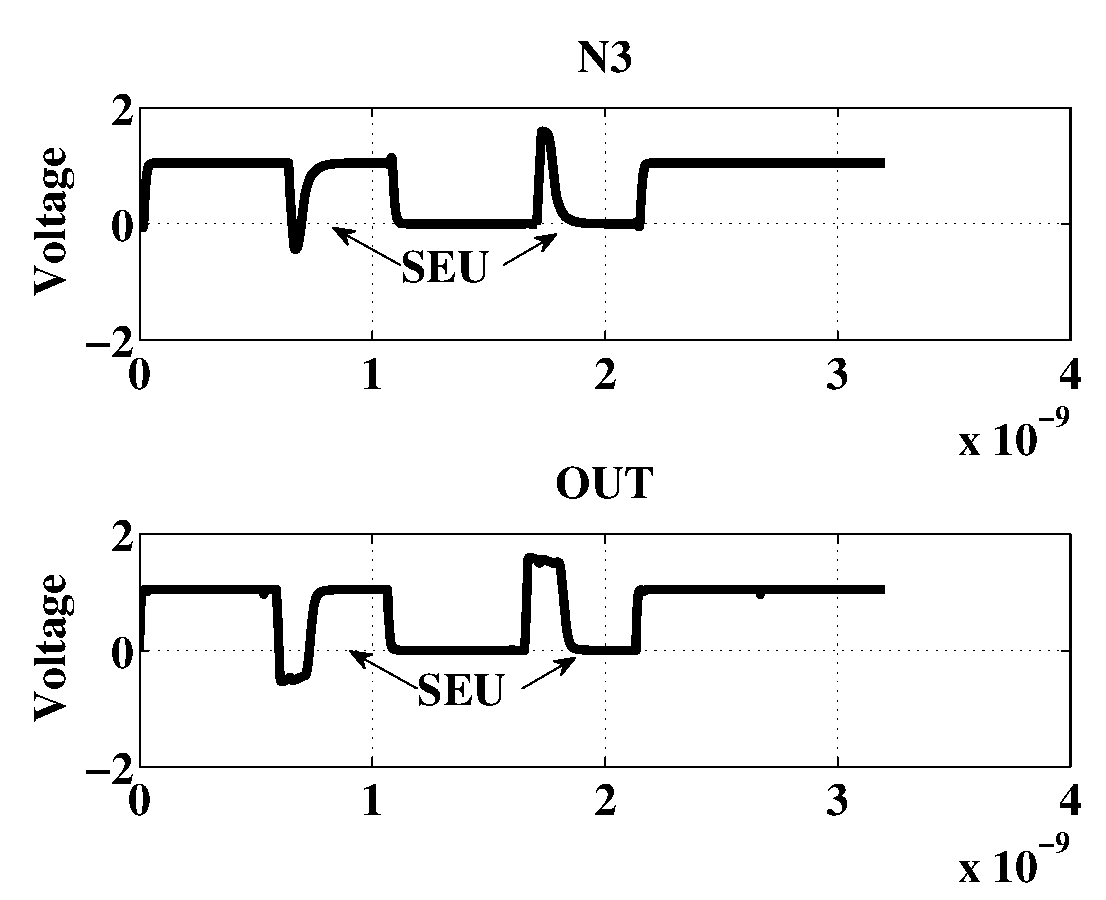
\includegraphics[width=\linewidth]{Figures/WavePlots/n3out.eps}
\caption{Node pair n3 and out upset and recovery.}
\label{fig:n5n6}
\end{minipage}
\end{figure}

Next, we compare the HRDNUT to existing SEU and DNU tolerant methods. As in the HRDNUT latch, all latches were designed using the 32nm PTM library and operated at 1Ghz. For the analysis, we compare to the following SEU tolerant latches: DICE \cite{DICE}, FERST \cite{FERST} and HIPER \cite{HIPER}. Additionally, we also compare to the following DNU tolerant designs: DNCS \cite{DNCS}, Interception \cite{Inter}, HSMUF \cite{HSMUF} and DONUT \cite{DONUT}. All transistors for the implemented latches were set to minimum width and length except for the designs that use a C-element with a weak keeper. In these designs the C-element's PMOS width was set to W=320nm and the NMOS width was set to W=160nm and the weak keeper was sized to be at minimum width. The C-element was sized so that the output driving strength did not allow the keeper to drive an erroneous value in the event of an error. 

To provide a fair comparison, we measure the propagation delay, average power consumption and area of all designs and categorize them base on whether they can tolerate a DNU and if they are robust from error after a DNU occurs. The delay was measured as the time between when a transition occurs on input \textit{D} to when a transition was observed on the output. The average power was computed using the error-free operation for each latch for a duration of 200ns. To compare the area overhead, we adopt the unit size transistor (UST) metric as in \cite{DNCS} which represents the number of unit sized (minimum width is W=40nm in this case) transistors required for the design. Table \ref{table:rtable} provides the results of these simulations.

\begin{table}[h]
\begin{center}
	\caption{SPICE Simulations of Existing Latches using the 1.05V 32nm PTM library }
	\label{table:rtable}
	\begin{tabular}{|m{5em}|m{3.5em}|m{3em}|m{3em}|m{3em}|m{3em}|}
	\hline
	Latch & DNU Immune & DNU Robust & Power ($\mu$W) & Delay (ps) & Area (UST)\\ 
	\hline
	DICE & No & No & 1.332 & 8.145 & 16 \\
	\hline
	FERST & No & No & 3.178 & 31.648 & 60 \\
	\hline
	HIPER & No & No & 1.292 & 2.221 & 27 \\
	\hhline{|=|=|=|=|=|=|}
	DNCS & Yes & No & 4.948 & 22.486 & 61 \\
	\hline
	\cite{Inter} & Yes & No & 5.606 & 79.168 & 89 \\
	\hline
	HSMUF & Yes & No & 1.871 & 1.0626 & 51 \\
	\hline
	HSMUF (Keeper) & Yes & No & 3.787 & 3.945 & 78 \\
	\hhline{|=|=|=|=|=|=|}
	DONUT \cite{DONUT} & Yes & Yes & 4.021 & 14.722 & 54 \\ 
	\hline
	DONUT-M (Section \ref{sec:DNUdes}) & Yes & Yes & 2.760 & 8.421 & 72\\
	\hline
	HRDNUT (Proposed) & Yes & Yes & 2.450 & 2.310 & 66 \\
	\hline
	\end{tabular}
\end{center}
\end{table}

According to Table \ref{table:rtable} the only DNU robust designs are the two DONUT latch implementations and the HRDNUT. Compared to the modified DONUT latch, the HRDNUT provides DNU robustness while reducing the power consumption and number of transistors by 11.3\% and 8.33\% respectively while also reducing the delay by 72.5\%. For the above reasons, the HRDNUT is the best design for clock gating applications due to its high robustness, even after a DNU occurs, and lower power, delay and area overheads.